\subsection{Gewählte Technologien}
\label{ssub:gewählte_technologien}
  Die auszuwählenden Technologien für ein solches Projekt sind zahlreich. Da es sich bei dieser Arbeit um keine Produktentwicklung mit eingeschränktem Nutzerkreis handelt, besteht bei der Technologieauswahl uneingeschränkte Freiheit. Um diesen Umstand auszunutzen und dem Projekt einen experimentellen Charakter zu verleihen, sollen vor allem zukunftsweisende Technologien Verwendung finden.
  
  \subsubsection{Datenbank}
  \label{ssub:datenbank}
    Da der GTFS-Standard eine fertige relationale Beziehung der einzelnen Dateien festlegt, ist der Einsatz einer relationalen Datenbank sehr naheliegend. Dabei gibt es eine breite Palette an Auswahl. Damit die Anwendung möglichst zugänglich bleibt, liegt der Fokus auf Datenbanken, die unter einer Open-source-Lizenz kostenfrei zur Verfügung stehen. Die zwei populärsten sind MySQL und PostgreSQL\parencite{db_engines}. Beide haben ihre Vor- und Nachteile und die Entscheidung ist mehr eine persönliche Präferenz, als ein großer Vorteil des Einen über den Anderen. Einen kleinen Vorteil bietet PostgreSQL's Unterstützung für Array-Types, welche sehr hilfreich beim Speichern und Abfragen von Daten ist. So fiel die Entscheidung auf die PostgreSQL Datenbank, wobei eine Realisierung auch mit MySQL möglich gewesen wäre.
  % subsubsection datenbank (end)

  \subsubsection{Serverwahl}
  \label{ssub:serverwahl}
    Für das Backend soll \texttt{Nodejs} verwendet werden. Nodejs ist nicht nur einfach aufzusetzen, sondern auch sehr performant und effizient für Web Applikationen einsetzbar. Zudem lässt es sich sehr einfach mittels Docker in der AWS (Amazon Web Services) Cloud veröffentlichen. Da Nodejs dynamisch typisiert, lassen sich vor allem auch Prototypen sehr schnell erstellen. Zusätzlich können sowohl Server und Client in JavaScript programmiert werden, wodurch die meisten Frameworks sowohl für den Server als auch für den Client zur Verfügung stehen.
  % subsubsection serverwahl (end)
  
  \subsubsection{Kartenmaterial}
  \label{ssub:kartenmaterial}
    Bereits zu Beginn wurde von einer hohen zu bewältigenden Datenmenge ausgegangen. Um die Voraussetzungen dafür zu schaffen, wurde nach Softwarelösungen gesucht, die für solche Datenmengen ausgelegt sind. Für die Karte wird dafür Mapbox eingesetzt. Mapbox verwendet Web-GL (basierend auf OpenGL) und bietet damit die Möglichkeit, ein GPU-unterstütztes Rendering im Browser zu ermöglichen. Zusätzlich bietet Mapbox gegenüber Google-Maps den Vorteil von eigene Karten-Styles. Diese können über Mapbox-Studio voll umfänglich auf die eigenen Bedürfnisse angepasst werden. Parks, Straßen, Schriftzüge, nahezu alle Elemente der Karte, lassen sich ändern und anpassen. Zusätzlich können eigene Daten in die Karte integrieren werden, was Bandbreite und Rechenleistung spart. Damit können sämtliche Routen, die das Stuttgart-VVS Feed beinhaltet, in das Kartenmaterial gezeichnet werden (siehe orangene Linien in Abbildung \ref{fig:map_tiles_routes}).

    \begin{figure}[htbp]
      \begin{center}
        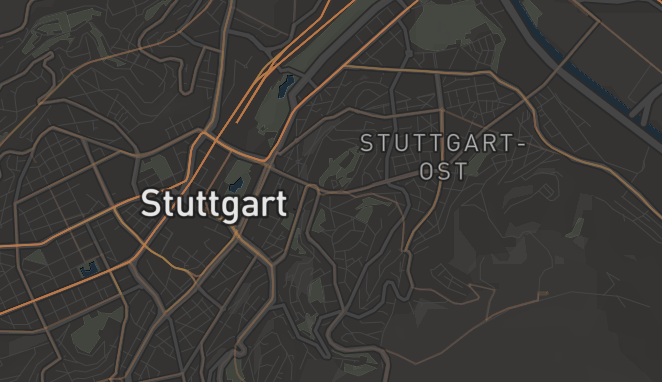
\includegraphics[width=0.5\textwidth]{map_tiles_routes}
        \caption{Karte mit integrierten Stuttgart-VVS Daten}
        \label{fig:map_tiles_routes}
      \end{center}
    \end{figure}
    
    Die Wahl der richtigen Tools ist dabei nur die Grundlage, um die Datenmenge zu bewältigenden. Viele weitere Schritte sind notwendig, um eine performante Webanwendung zu erstellen und werden in im nächsten Kapitel \nameref{sec:develop} noch ausführlicher aufgeführt.
    
  % subsubsection kartenmaterial (end)

  \subsubsection{Frameworks}
  \label{ssub:frameworks}
    Für die Programmierung wurden folgende Bibliotheken ausgewählt. Diese bieten verschiedenste Erleichterungen bei der Programmierung.

    \begin{itemize}[label={}]
      \item \textbf{Turf}\footnote{\url{http://turfjs.org/docs/}} stellt eine ganze Reihe an Funktionen für die raumbezogene Verarbeitung von Daten zur Verfügung. Beispielsweise lassen sich mittels Turf unter anderem Distanzen, Flächen oder Schnittpunkte berechnen.

      \item \textbf{Mapbox-gl-js}\footnote{\url{https://www.mapbox.com/mapbox-gl-js/api/}} wird benötigt, um das Kartenmaterial von Mapbox im Client zu verwenden. Dafür stellt es eine eigene API zur Verfügung.

      \item \textbf{Lodash}\footnote{\url{https://lodash.com/}} ist eine Hilfsbibliothek, die verschiedene Funktionen zur Verfügung stellt, die das Arbeiten mit JavaScript vereinfachen.

      \item \textbf{Express}\footnote{\url{https://expressjs.com/en/starter/basic-routing.html}} ist ein minimalistisches Node.js-Framework für moderne Web-Applikationen. Es vereinfacht die Erstellung von API-Endpunkten durch das Bereitstellen hilfreicher Methoden zur Erstellung des Routing. Routing bezieht sich dabei auf die Bestimmung, wie eine Anwendung auf eine Client-Anfrage an einen bestimmten Endpunkt reagiert, also auf eine URI (oder einen Pfad) und eine bestimmte HTTP-Request-Methode (GET, POST usw.).
    \end{itemize}
    
  % subsubsection frameworks (end)
% subsubsection gewählte_technologien (end)